\chapter{Newton's Laws of Motion}
\section{Space, Time, Mass, and Force}
Newton's laws of motion are formulated in terms of four crucial concepts: space, time, mass, and force. We will briefly review these 
concepts here. 

\subsection*{Space}
Every point $P$ of the three-dimensional space in which we live can be represented with a position vector $\bm{r}$ that specifies the distance and direction of $P$ from a chosen origin $O$. We can represent a position vector by expressing its components $(x,y,z)$ in the direction of three given perpendicular axes. One popular choice of axes is described by the unit vectors $\xhat$, $\yhat$, and $\zhat$, which have a length of one and point along the $x$, $y$, and $z$ axes. We can then write 
\begin{equation} \label{unit_vectors}
    \mbf{r} = x\xhat + y\yhat + z\zhat
\end{equation}
Some texts may use the equivalent notation of $\mbf{i}$, $\mbf{j}$, and $\mbf{k}$. Different authors have different preferences, so it will be helpful to get used to working with several notations.

We sometimes abbreviate (\ref{unit_vectors}) by simply writing
\begin{equation} \label{abb_vector}
    \mbf{r} = (x,y,z)
\end{equation}
When the choice of unit vectors is clear from the context. For most vectors, we will indicate the components of the vector with the subscripts $x$, $y$, and $z$. For instance, the velocity vector $\mbf{v}$ has components $v_x$, $v_y$, and $v_z$.

Sometimes, it become convenient to write vectors even more concisely using the summation sign $\sum$. In these cases, we will rename the unit vectors $\xhat$, $\yhat$, and $\zhat$ to $\mbf{e_1}$, $\mbf{e_2}$, and $\mbf{e_3}$ and we will rename the components $x$, $y$, and $z$ to $r_1$, $r_2$, and $r_3$. With this notation, we can write
\[ \mbf{r} = r_1\mbf{e_1} + r_2\mbf{e_2} + r_3\mbf{e_3} = \sum_{i=1}^3 r_i\mbf{e_i} \]

\subsection*{Time}
In classical mechanics, we view time as one universal parameter--that is, all objects will experience the flow of time at precisely the same rate. The theory of relativity states that this is not quite correct, which gives rise to phenomena such as length contraction and time dilation. However, for objects whose velocity is much less than the speed of light, these effects are negligible and we will ignore them.

\subsection*{Reference Frames}
Every time we wish to solve a problem in physics, we will have to choose a \it{reference frame}. Reference frames give a choice of spatial origin and axes, as well as an origin for time. Choosing an appropriate reference frame will simplify calculations for many problems, and is a skill that will be vital to build.

When choosing a reference frame, it will be important to note the difference between \it{inertial} reference frames and non-inertial ones. This is because Newton's laws of motion will only hold true in inertial reference frames. 

Any frame of reference that is accelerating or rotating relative to an inertial frame is non-inertial. Studying non-inertial frames will require more advanced techniques than we currently have, so we will focus solely on inertial frames for the time being.

\subsection*{Mass}
The mass of an object characterizes its inertia, or resistance to movement. An object with a large amount of mass, like a boulder, will be harder to accelerate than an object with less mass, like a marble.

\subsection*{Force}
Informally, we think of a force as a push or a pull on an object. This is a surprisingly useful starting point, as we are typically very conscious of the forces we exert on the world and the world exerts on us. Forces are vector quantities that can be represented as
\[ \mbf{F} = F_x\xhat + F_y\yhat + F_z\zhat \]
We can also represent the magnitude of a force with $F = \sqrt{F_x^2 + F_y^2 + F_z^2}$. 

\section{Newton's First and Second Laws; Inertial Frames}
Throughout this chapter, we will discuss Newton's laws as they apply to a \bf{point mass}. A point mass is a ficticious construct of an object with mass, but no size. Of course, all objects have some sort of size--but many objects are so small that treating them as a point mass will not cause any issues. Later, we will explore the mechanics of extended bodies by representing them as a collection of many point masses.

The first two of Newton's laws are easily stated and well-known.

\begin{theorem}[Newton's First Law]
    Newton's first law tells us that in the absence of forces, a particle moves with a constant velocity $\mbf{v}$.
\end{theorem}
\begin{theorem}[Newton's Second Law]
    Newton's second law tells us that the net force $\mbf{F}$ is equal to the product of its mass $m$ and its acceleration $\mbf{a}$:
    \[ \mbf{F} = m\mbf{a} \]
\end{theorem}
We will introduce the notation $\mbf{a} = \mbf{\dot v} =  \mbf{\ddot{r}}$, where each dot represents the operation of differentiation with respect to $t$. This means that we can also write $\mbf{F} = m\mbf{\ddot{r}}$.

Alternatively, we can write Newton's second law in terms of the particle's \bf{momentum}. Momentum is a vector quantity defined as
\[ \mbf{p} = m\mbf{v} \]
Thus, $\mbf{\dot p} = m\mbf{\dot v} = m\mbf{a}$, so we can state
\[ \mbf{F} = \mbf{\dot p} \]
\subsection*{Differential Equations}
In the form $\mbf{F} = m\mbf{\ddot r}$, Newton's second law is a second order differential equation (or perhaps a higher order one if $\mbf{F}$ depends on higher derivatives of $\mbf{r}$) describing the position $\mbf{r}(t)$ of the particle. 

This representation gives us a few key insights about a particle. These insights draw from the theory of differential equations, and may be explained in more detail in a text dedicated to that theory.

\begin{enumerate}
    \item If the force can be described as a piecewise-continuous function of $\mbf{r}$ and its derivatives and $t$, then a family of functions describing posisble positions $\mbf{r}(t)$ can be found.
    \item The family of position functions can be narrowed down to one unique position function using a pair initial conditions $\mbf{r}(t_0) = \mbf{r_0}$ and $\mbf{r}'(t_0) = \mbf{r_0'}$.
    \item If $\mbf{F}$ depends on higher order derivatives of $\mbf{r}$, more initial conditions will be required as the equation will increase in order.
\end{enumerate}

\subsection*{Inertial Frames}
Previously, we said that Newton's laws do not hold up in non-inertial reference frames. To see this, consider some frame $\mathcal{S}$ where Newton's laws hold. $\mathcal{S}$ is then an inertial frame. If we consider some other frame $\mathcal{S}'$ that is moving at a constant velocity in a straight line relative to $\mathcal{S}$, we'll notice that any object that isn't accelerating in $\mathcal{S}$ is also not accelerating in $\mathcal{S}'$. Therefore the law of inertia holds in $\mathcal{S}'$ and so $\mathcal{S}'$ is also inertial. 

If we consider a third frame $\mathcal{S}''$ that is accelerating relative to $\mathcal{S}$, then any object moving at a constant velocity in $\mathcal{S}$ is accelerating in $\mathcal{S}''$. The amount of acceleration it has is equal to the amount $\mathcal{S}''$ is accelerating relative to $\mathcal{S}$, but in the opposite direction.

For the time being, we will just consider the mechanics of objects in inertial reference frames, but we will explore noninertial frames in more detail later on.

\subsection*{Validity of the First Two Laws}
Since the advent of relativity and quantum mechanics, we have known that Newton's laws are not universally valid. However, there are still many cases where they are. Even as the speed of objects approaches the speed of light $c$, the law of inertia remains completely valid. But in these cases, the second law $\mbf{F} = m\mbf{a}$ is no longer valid and we must instead use $\mbf{F} = \mbf{\dot p}$.

The main takewaway here is that for most scenarios we will be working with, the first two laws are completely valid.
\section{Newton's Third Law}
Every force that is exerted on an object will always involve a second force--the reaction force back onto the object that exerts the force. When you push on a wall, the wall pushes back (otherwise you'd just fall right through). 

So forces come in pairs. We will introduce a new notation $\mbf{F}_{21}$ to denote the force exerted on object 2 by object 1. Similarly, $\mbf{F}_{12}$ denotes the force exerted on object 1 by object 2. With this notation, we can express Newton's third law quite compactly. 

\begin{theorem}[Newton's Third Law]
    If object 1 exerts a force $\mbf{F}_{21}$ on object 2, then object 2 exerts a reaction force $\mbf{F}_{12}$ on object 1 given by
    \begin{equation}
        \mbf{F}_{12} = -\mbf{F}_{21}
    \end{equation}
\end{theorem}
In the special case where $\mbf{F}_{12}$ an $\mbf{F}_{21}$ act parallel to the line connecting object 1 and object 2, we call them \bf{central forces}. Many of the most common forces we encounter are central forces: gravity, the electrostatic force, etc.

Newton's third law has a nice connection with the law of conservation of momentum. Imagine two objects that exert forces $\mbf{F}_{12}$ and $\mbf{F}_{21}$ on each other, and perhaps have some other external forces acting on them. The net force on each object can be expressed as 
\[ \mbf{F}_1 = \mbf{F}_{12} + \mbf{F}^{\text{ext}}_1 \]
and
\[ \mbf{F}_2 = \mbf{F}_{21} + \mbf{F}^{\text{ext}}_2 \]
which, by Newton's second law, tells us that $\mbf{\dot p}_1 = \mbf{F}_{12} + \mbf{F}^{\text{ext}}_1$ and $\mbf{\dot p}_2 = \mbf{F}_{21} + \mbf{F}^{\text{ext}}_2$. The total momentum of the system is the sum of each individual objects' momentum $\mbf{P} = \mbf{p}_1 + \mbf{p}_2$. Thus
\begin{align*}
    \mbf{\dot P} &= \mbf{\dot p}_1 + \mbf{\dot p}_2 \\
    &= \mbf{F}_{12} + \mbf{F}^{\text{ext}}_1 + \mbf{F}_{21} + \mbf{F}^{\text{ext}}_2
\end{align*}
By Newton's third law, $\mbf{F}_{12} = -\mbf{F}_{21}$ so they cancel out, simply leaving us with
\[ \mbf{\dot P} = \mbf{F}^{\text{ext}}_1 + \mbf{F}^{\text{ext}}_2 \equiv \mbf{F}^{\text{ext}}\]
This leads to a critical observation for our two-particle system--if the net external force on the system is zero, then the total momentum of the system is constant.

We will now show that the same result holds for any $N$-particle system.

Consider a system of $N$ particles where the net force on particle $i$ is given by
\[ \mbf{F}_i = \mbf{\dot p}_i = \mbf{F}^{\text{ext}}_i + \sum_{j \neq i} \mbf{F}_{ij}\]
The sum rate of change of the momentum of the system is the sum of each of these net forces,
\begin{align*}
    \mbf{\dot P} &= \sum_{i} \mbf{\dot p}_i  \\
    &= \sum_{i} \pqty{ \mbf{F}^{\text{ext}}_i + \sum_{j \neq i} \mbf{F}_{ij}} \\
    &= \mbf{F}^{\text{ext}} + \sum_{i}\sum_{j \neq i} \mbf{F}_{ij}
\end{align*}
The second term consists of $N+(N-1)$ terms and can be split into $n(n-1)/2$ pairs of forces that cancel with each other. We can show this mathematically with a manipulation of the summation. 
\[\sum_{i}\sum_{j \neq i} \mbf{F}_{ij} = \sum_{i}\sum_{j < i}(\mbf{F}_{ij} + \mbf{F}_{ji}) = 0 \]
Therefore the total rate of change of momentum on the system is given by
\[ \mbf{\dot P} = \mbf{F}^{\text{ext}} \]
Now we can make a more general statement of the principle of conservation of momentum.
\begin{theorem}[Conservation of Momentum]
    If the net external force $\mbf{F}^{\text{ext}}$ on an $N$-particle system is zero, then the system's total momentum is constant.
\end{theorem}
\subsection*{Validity of Newton's Third Law}
Similar to Newton's first and second laws, the third law is not universally applicable. As speeds of objects approach $c$, the third law cannot hold because the time-dependent action and reaction forces $\mbf{F}_1(t)$ and $\mbf{F}_2(t)$ for two objects differ depending on the speed of the observer, even if their frame of reference is inertial.

There is also an example of a quite common force where Newton's third law doesn't hold: the magnetic force between two moving point charges. 

Consider two positively charged particles, one with charge $q_1$ moving in the $\xhat$ direction and one with charge $q_2$ moving in the $\yhat$ direction. As per the Biot-Savart law, the direction of the magnetic field $\mbf{B_2}$ created by $q_1$ at the location of $q_2$ is given by 
\[ \mbf{B_2} \propto \mbf{\dot r}_1 \times \mbf{\hat d} \]
where $\mbf{d}$ is the displacement vector between $q_1$ and $q_2$. $\mbf{\dot r}_1$ is in the $\xhat$ direction and $\mbf{d}$ is in the $\xhat$-$\yhat$ plane, so $\mbf{B_2}$ lies one the $\zhat$ axis.

A similar argument shows that $\mbf{B_1}$ is in the \textit{negative} $\zhat$ direction. 

Then, the magnetic component of the Lorentz force for each particle is given by
\begin{align*}
    \mbf{F}_{B,1} = \mbf{F}_{12} &= q_1\mbf{\dot r_1}\times \mbf{B_1}\\
    &= q_1\dot r_1 B_1 (\xhat \times \zhat) \\
    &= q_1\dot r_1B_1 \yhat
\end{align*}
and
\begin{align*}
    \mbf{F}_{B,2} = \mbf{F}_{21} &= q_2\mbf{\dot r_2}\times \mbf{B_2}\\
    &= q_2\dot r_2 B_2 (\yhat \times -\zhat) \\
    &= q_1\dot r_2B_2 \xhat 
\end{align*}
clearly, these forces do not act in opposite directions, violating Newton's third law.

Because we have shown that the statement of conservation of momentum is equivalent to the statement of Newton's third law, this result seem to imply that the magnetic force does not obey the conservation of momentum.

This error comes from the fact that the introductory physics view of electromagnetism does not portray the full picture of electromagnetic interactions. In fact, the lost momentum in the two particles is actually stored within the electromagnetic fields themselves.

It can be shown that for a particles moving with speeds $v_1$ and $v_2$, the magnitude of the electric force between the particles is greater than or equal to $v_1v_2/c^2$ times the magnetic force. Therefore the magnetic force can be taken to be negligible compared to the electric force and the lost mechanical momentum can be safely disregarded for low speeds.

\section{Newton's Second Law in Cartesian Coordinates}
We will now see how we can use the relationship $\mbf{F} = m\mbf{\ddot r}$ to solve for the motion of objects. This relationship can be split into a separate equation for each direction with the expansion
\[ \mbf{F} = F_x\xhat + F_y\yhat + F_z\zhat \]
and
\[ \mbf{\ddot r} = \ddot x\xhat + \ddot y\yhat + \ddot z\zhat \]
thus giving the three equations of motion
\[ F_x = m\ddot x \quad F_y = m\ddot y \quad F_z = m\ddot z \]
Generally, when we solve a problem of this form we will qualitatively analyze the situation to determine each force present on the object, and then solve the corresponding system of differential equations. 
\begin{example}[Inclined Plane] \label{inclined}
    A block of mass $m$ begins at rest on an inline with a coefficient of friction $\mu$ that rests at an angle $\theta$ above the horizontal floor. Determine an expression for how far the block will slide during a certain time $t$.
    
    \begin{minipage}{0.48\textwidth}
        As with any mechanics problem, we will begin by defining our frame of reference. We will choose the origin point of our coordinate system to be at the initial position of the block, and we will define the $\xhat$ direction as going down the slope of the incline, and the $\yhat$ direction as protruding upward from the incline at a $90$ degree angle. We will define the $\zhat$ direction as the direction given by $\xhat \times \yhat$, but this will prove to be irrelevant as no forces act in that direction.
    \end{minipage}
    \begin{minipage}{0.48\textwidth}
        \parbox{\textwidth}{
            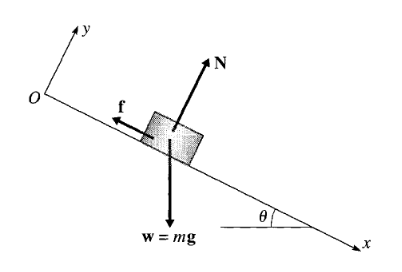
\includegraphics[width=\textwidth]{blockSlidingExample.png}
        }
    \end{minipage}
    
    This is a particularly useful frame of reference because it ensures that the friction force and normal force both lie in the direction of one of our basis vectors.

    From the figure and a relatively simple exercise in trigonometry, we can determine the directions of each force. The frictional force $\mbf{f}$ acts purely in the $-\xhat$ direction, the normal force $\mbf{N}$ acts purely in the $\yhat$ direction, and the weight force $\mbf{w}$ has components in both directions, with relative magnitudes given by
    \[ \mbf{w} = w\sin\theta\xhat - w\cos\theta\yhat\]
    So the net force on the object is given by
    \[ \mbf{F} = (mg\sin\theta - \mu N)\xhat + (N - mg\cos\theta)\yhat\]
    Because the block is not accelerating at all in the $\yhat$ direction, the component of $\mbf{F}$ in the $\yhat$ direction must be zero, telling us that
    \[ N - mg\cos\theta = 0\]
    or $N = mg\cos\theta$. Substituting this back into the expression for $F_x$, we get
    \[ F_x = mg\sin\theta - \mu mg \cos\theta \]
    By Newton's Second Law, this gives us the differential equation
    \[ \ddot x = g\sin\theta - \mu g\cos \theta \]
    Which can be solved by integrating twice to find 
    \[ x(t) = \frac{1}{2}g(\sin\theta-\mu\cos\theta)t^2 \]
    Both constants of integration are simply zero due to the prescribed initial condition $x(0)=x'(0) = 0$.
\end{example}
\section{Two Dimensional Polar Coordinates}
Cartesian coordinates are very simple to work with, but there are many cases where polar coordinates prove more effective. Recall from introductory Calculus that polar coordinates can be related to recangular coordinates with
\[ 
\begin{rcases}
    x = r\cos\phi \\
    y = r\sin\phi
\end{rcases} \longleftrightarrow \begin{cases}
    r = \sqrt{x^2+y^2} \\
    \tan\phi = y/x
\end{cases}
\]
In physics, it is common to use $\phi$ as the polar angle rather than $\theta$. One thing to note is the possible ambiguity in the expression $\tan\phi = y/x$. Because $\tan(y/x) = \tan(-y/-x)$ and $\tan(-y/x) = \tan(y/-x)$, we will have to be careful to find the correct quadrant of $\phi$ when converting from rectangular to polar coordinates.

Just as in rectangular coordinates, we introduce two unit vectors $\rhat$ and $\phihat$. $\rhat$ is defined as the direction we move as $r$ increases while $\phi$ is held constant, and $\phihat$ is defined as the direction we move as $\phi$ increases while $r$ is held constant. 

These two unit vectors form an orthonormal basis for $\R^2$ and we can expand forces in terms of them as
\[ \mbf{F} = F_r\rhat + F_\phi \phihat\]
We can also note that $\mbf{r} = r\rhat$. Initially, it seems odd that the position vector has no explicit dependence on $\phi$. The dependence actually originates from the unit vector $\rhat$. Unlike the unit vectors in cartesian coordinates, the polar unit vectors are not constant, and depend on the state of the system. 

This revelation complicates our expression of Newton's Second Law in polar, as 
\[ \ddot r = \dv[2]{t}(r\rhat) \neq r\mbf{\ddot{\hat r}}\]
To resolve this, we'll draw a picture.

Suppose a particle is at a position $r\rhat + \phi\phihat$ at time $t_1$ and a position $(r + \Delta r)(\rhat + \Delta\rhat) + (\phi + \Delta \phi)(\phihat + \Delta\phihat)$ at $t_2 = t_1 + \Delta t$. Notice from the below figure that $\Delta \rhat$ is not dependent on $\Delta r$, so we will assume it is zero, so
\[ \mbf{r}(t_2) = r(\rhat + \Delta \rhat) + (\phi + \Delta \phi)(\phihat + \Delta \phihat)\]
\begin{figure}[h!]
    \centering
    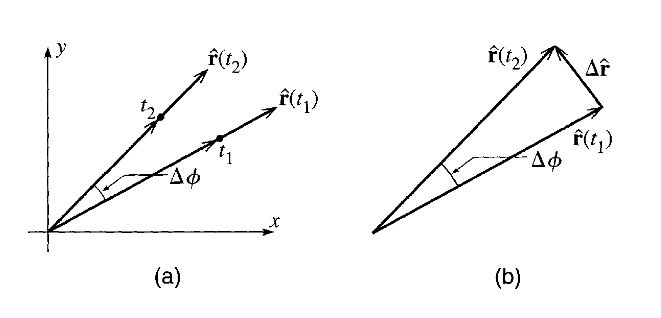
\includegraphics[width=0.65\linewidth]{polarDerivatives.png}
    \caption{\bf{(a)} Unless the particle is moving completely radially, the $\rhat$ vectors differ at $t=t_1$ and $t=t_2$. \bf{(b)} The change $\Delta \rhat$ is given by the pictured triangle.}
    \label{fig:polarDerivatives}
\end{figure}

As shown in part \bf{(b)} of the above figure, $\Delta \rhat$ is described by the triangle with an angle $\Delta \phi$ and two sidelengths of length one (since each $\rhat$ satisfies $\norm{\rhat} = 1$). We can use some geometry to find $\Delta \rhat$. The law of cosines tells us that
\[ \norm{\Delta \rhat} = \sqrt{2 - 2\cos\Delta\phi}\]
With the small-angle approximation 
\begin{equation} \label{small_angle_polar_unit}
    \cos\Delta\phi \approx 1 - \frac{\Delta \phi ^2}{2}
\end{equation}
we obtain
\[ \norm{\Delta\rhat} \approx \abs{\Delta\phi} \]
We can also see from ($\ref{fig:polarDerivatives}$b) that $\Delta \rhat$ points in the direction of $\phihat(t_1)$. Therefore,
\[ \Delta \rhat \approx \Delta \phi \phihat(t_1) \]
or
\[ \frac{\Delta \rhat}{\Delta t} \approx \frac{\Delta \phi}{\Delta t} \phihat(t_1) \]
as $\Delta t\to 0$, this approximation becomes better and turns into
\[ \dotunit{r} = \dot{\phi}\phihat\]
With this, we can differentiate $\mbf{r} = r\rhat$ to obtain
\[ \mbf{v}\equiv \mbf{\dot r} = \dot{r}\rhat + r\dot{\phi}\phihat\]
We will sometimes write $\dot\phi$ as $\omega$, which denotes the angular velocity. This gives
\begin{equation} \label{polar_velocity}
    \mbf{v}  = \dot{r}\rhat + r\omega \phihat
\end{equation}
Before we can write Newton's Second Law, we will have to determine $\mbf{a}\equiv \ddot{r}$. Applying the product rule to (\ref{polar_velocity}),
\begin{equation} \label{polar_a_unsimplified}
    \mbf{a} = \ddot{r}\rhat + \dot{r}\dotunit{r} + \dot{r} \dot{\phi} \phihat + r \ddot{\phi}\phihat + r\dot{\phi}\dotunit{\phi}
\end{equation}
We already found that $\dotunit{r} = \dot{\phi}\phihat$, but we don't know what to replace $\dotunit{\phi}$ with. Consider the below figure. 
\clearpage
\begin{figure}[t]
    \centering
    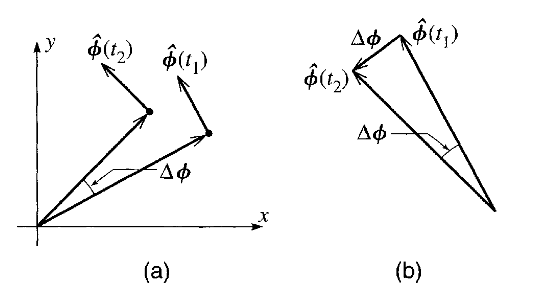
\includegraphics[width=0.65\linewidth]{polarDerivatives2.png}
    \caption{\bf{(a)} $\Delta \phihat$ is solely dependent on $\Delta\phi$. \bf{(b)} $\Delta\phihat$ is determined by the pictured triangle.}
    \label{fig:polarDerivatives2}
\end{figure}

We can use the law of cosines once again to see
\[ \abs{\Delta\phihat} = \sqrt{2-2\cos\Delta\phi} \]
which, using the same approximation as (\ref{small_angle_polar_unit}), we once find $\abs{\Delta \phihat} \approx \Delta \phi$. By placing the tip of $\phihat(t_1)$ at the tip of $\phihat(t_2)$, we can subtract them geometrically and convince ourselves that $\Delta \phihat$ points in the direction $-\rhat$. Thus, we obtain
\[ \Delta\phihat \approx -\Delta \phi \rhat(t_1)\]
or
\[ \frac{\Delta \phihat}{\Delta t} \approx -\frac{\Delta \phi}{\Delta t}\rhat(t_1)\]
once again taking the limit as $\Delta t\to 0$, we get
\[ \dotunit{\phi} = -\dot \phi \rhat\]
Substituting this and $\dotunit{r} = \dot{\phi}\phihat$ into (\ref{polar_a_unsimplified}), we find
\begin{equation} \label{polaracceleration}
    \mbf{a} = \pqty{\ddot r - r\dot{\phi}^2}\rhat + \pqty{2\dot{r}\dot\phi + r\ddot{\phi}}\phihat
\end{equation}
This result in its full generality is quite difficult to interpret, so we will consider the special case where $r$ is fixed. This means that $\dot r = \ddot r = 0$, so
\[ \mbf{a} = -r\dot{\phi}^2\rhat + r\ddot{\phi}\phihat \]
or
\[ \mbf{a} = -r\omega^2\rhat + r\alpha \phihat\]
where $\omega = \dot r$ is defined as before and $\alpha = \ddot r$ is the angular acceleration. This describes the common result from elementary physics that an object moving in circular motion with a fixed radius has an inward radial ``centripetal" acceleration given by $r\omega^2 = v^2/r$ and a tangential acceleration $r\alpha$.

With (\ref{polaracceleration}), we can now write down Newton's Second Law in polar form:
\[ \mbf F = m\mbf{a} = (m\ddot r - mr\dot{\phi}^2)\rhat + (mr\ddot \phi + 2\dot{r}\dot{\phi})\phihat\]
\begin{example}[An Oscillating Skateboard]
    A smooth half-pipe at a skate park consists of a concrete trough with a semicircular cross section of radius $R$. A skateboard is released from rest at an angle $\phi=\phi_0$ from the vertical. Determine an expression for the movement of the skateboard as $t$ varies, and determine when the skateboard returns to its original position.   
    
    \begin{minipage}{0.48\textwidth}
        This is a problem where polar coordinates will prove extremely useful. We will define the origin $O$ aligned vertically with the top of the half-pipe and aligned horizontally with the middle of it, as shown in the figure to the right. We will also define $\phi=0$ to be the line pointing straight down, with counterclockwise being the direction of increasing $\phi$.
    \end{minipage}
    \begin{minipage}{0.48\textwidth}
        \parbox{\textwidth}{
            \label{half-pipe}
            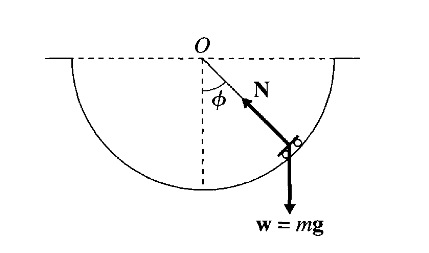
\includegraphics[width=\textwidth]{halfPipe.png}
        }
    \end{minipage}
    
    Because the radius is held constant at $r=R$, Newton's Second law tells us 
    \[ \mbf{F} = -mR\dot{\phi}^2\rhat + mR\ddot{\phi}\phihat \]
    The two forces on the skateboard are the weight force $\mbf{w}$ and the normal force $\mbf{N}$. $\mbf{N}$ acts solely in the $-\rhat$ direction. With some trigonometry, we can determine that $\mbf{w} = mg\cos\phi\rhat - mg\sin\phi\phihat$. Thus the motion of the skateboard is determined by the equations
    \[ -mR\dot{\phi}^2 = mg\cos\phi - N \quad \text{and} \quad mR\ddot{\phi} = -mg\sin\phi\]
    We aren't particularly interested in the left equation, as we are able to fully solve for the motion with just the one on the right. We can rearrange to obtain
    \[ \ddot\phi = -\frac{g}{R}\sin\phi \]
    which is a second order differential equation for $\phi$. Due to the nonlinearity of this equation, it is impossible to solve in terms of elementary functions. Instead, we will make the approximation $\sin\phi\approx\phi$ to find 
    \[ \ddot\phi = -\frac{g}{R}\phi \]
    We will define a quantity $\omega = \sqrt{g/R}$ as the \textit{angular frequency} of the oscillation, and then the general solution is given by
    \[ \phi(t) = A\sin(\omega t) + B\cos(\omega t)\]
    With the initial condition $\phi(0) = \phi_0$ and $\phi'(0)=0$, obtain a particular solution given by
    \[ \phi(t) = \phi_0\cos(\omega t)\]
    To determine how long it will take for the skateboard to return to its original position, we will rely on the periodicity of the cosine function. If $\phi_0\cos(\omega t) = \phi_0$, then we must have $\omega t = 2\pi n$ for some natural number $n$. The earliest such time besides $t=0$ is given by choosing $n=1$, so $t = 2\pi/\omega$. 

    We call this time the \textit{period} of the oscillation, and denote it with $\tau$.

    \begin{minipage}{0.48\textwidth}
    While the approximation $\sin\phi\approx\phi$ is remarkably effective for relatively small $\phi$, it is important to note that it is only an approximation. If we have a large initial condition, such as $\phi_0 = \pi/3$, the small angle approximation is no longer accurate and will lead to significant deviation between the approximated solution and the real solution. For an example of this, see the figure on the right, which plots $\phi$ versus $t$ for $R=5$ and $\phi_0 = \pi/3$. Clearly, there is significant error between the approximated solution (blue), and the true solution (red), which was obtained via numerical methods.
    \end{minipage}
    \begin{minipage}{0.48\textwidth}
        \parbox{\textwidth}{
            \label{error}
            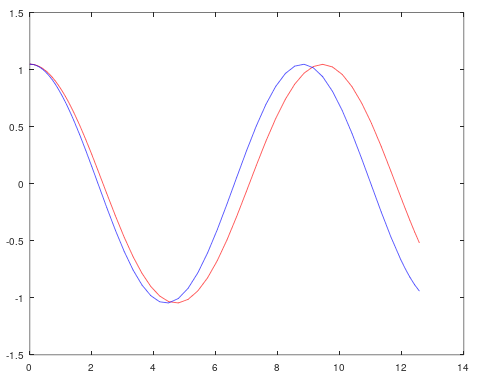
\includegraphics[width=\textwidth]{approximationError.png}
        }
    \end{minipage}
\end{example}
